%%%%%%%%%%%%%%%%%%%%%% PREAMBULE %%%%%%%%%%%%%%%%%%%%%%%%%%%%%%%%%%%%%%%%

%%%%%%%%%%%%%%%% PARAMETRES DU DOCUMENT %%%%%%%%%%%%%%%%%%%%%%%%%%%%%%%%%
\documentclass[12pt,a4paper]{article}
\usepackage[utf8]{inputenc}
\usepackage[T1]{fontenc}
\usepackage[french]{babel}

%%%%%%%%%%%%%%%%%%%%% PACKAGES %%%%%%%%%%%%%%%%%%%%%%%%%%%%%%%%%%%%%%%%%%
\usepackage{hyperref}
\usepackage{shorttoc}
\setlength{\parindent}{0pt}
\usepackage[top=2cm,bottom=2cm,right=2cm,left=2cm]{geometry}
\usepackage{multicol}
\usepackage{nccrules}
\usepackage{eurosym}
\usepackage{listings}
\usepackage{caption}
\usepackage{makecell}
\usepackage{graphicx}
\usepackage{subfigure}
\usepackage{hyperref}
\usepackage{biblatex}
\addbibresource{biblio.bib}
\usepackage{listings}
%\usepackage{minipage}
%%%%%%%%%%%%%%%%%%%%%%%%%%%%%%%%%%%%%%%%%%%%%%%%%%%%%%%%%%%%%%%%%%%%%%%%%


%%%%%%%%%%%%%%% PARAMETRAGES PACKAGES %%%%%%%%%%%%%%%%%%%%%%%%%%%%%%%%%%%
\captionsetup{labelformat=empty}

\hypersetup{
	colorlinks=true,
	linkcolor=blue,
	urlcolor=blue,
	citecolor=black
	}

%%%%%%%%%%%%%%%%%%%%%%%%%%%%%%%%%%%%%%%%%%%%%%%%%%%%%%%%%%%%%%%%%%%%%%%%%

\setlength{\fboxrule}{.2pt}

%%%%% PAGE DE TITRE %%%%
\title{UE L318 - Semaine 1}

\author{Hugo Lignères}

\date{22/02/2025}

\begin{document}

\maketitle

\hrulefill
\vspace{6cm}
\begin{center}
	
\includegraphics[scale=.4]{../images/univ.png}
		\\
		\vspace{2cm}
	
\includegraphics[scale=.25]{../images/cvtic.png}
\end{center}

%%%%%%%%%%%%%%%%%%%%%%%%%%%%%%%%%%%%%%%%%%%%%%%%%%%%%%%%%%%%%%%%%%%%%%%%%%

\newpage

\tableofcontents

\newpage

\section{DNS}

	\subsection{Le protocole DNS en détail}
	
	Le \textbf{Domain Name System} est un protocole qui permet de traduire le nom de domaine d'un site web en adresse IP qu'un serveur peut comprendre. \\
	
	Son architecture est la suivante : \\
	\begin{itemize}
		\item[1.] \textbf{Résolveur DNS} $\rightarrow$ Reçoit et gère les requêtes DNS qui proviennent de la machine côté client. Ensuite, il entre en contact avec les serveurs DNS pour traduire le nom de domaine en adresse IP ;
		\item[2.] \textbf{Serveurs racines} $\rightarrow$ Points d'entrée d'une résolution DNS. Ces serveurs sont au nombre de 13. Ils redirigent les requêtes vers les serveurs TLD adéquats ;
		\item[3.] \textbf{Serveurs TLD (Top-Level Domain} $\rightarrow$ Ils gèrent les noms de domaines comme \texttt{.com}, \texttt{.net}, \texttt{.org}, etc.
		\item[4.] \textbf{Serveurs de noms} $\rightarrow$ Ces serveurs contiennent des enregistrements DNS pour des noms de domaine spécifiques. 
		\item[5.] \textbf{Enregistrements DNS} $\rightarrow$ Ce sont des entrées stockées dans une base de données DNS qui contiennent des informations sur des noms de domaine et leurs adresses IP correspondantes ;
		
	\end{itemize}
	
	\subsection{Les détournements DNS}
	
	
		\subsubsection{DNS Hijacking}
		
		Cette attaque consiste à modifier les enregistrements DNS d'un domaine, afin de rediriger le traffic vers des sites malveillants. Le plus souvent, ces attaques se produisent en corrompant les registres DNS d'un domaine, d'un serveur ou d'un routeur. \\
		
		Tout simplement, un attaquant infiltre un ou plusieurs serveurs d'un site souvent visité, pour rediriger les utilisateurs vers des sites malveillants, souvent contrôlés par les attaquants.
		
		
		\subsubsection{Man-in-the-Middle}	
		
		Un attaquant intercepte des requêtes et réponses DNS, pour altérer les informations contenues dans ces dernières, et renvoyer les utilisateurs vers d'autres sites, souvent malveillants. \\
		
		Un exemple courant est de créer un faux point d'accès wi-fi gratuit dans un espace publique (aéroport, gare, restaurant, parc, etc), pour intercepter le traffic DNS des utilisateurs connectés. Il peut ensuite rediriger ces utilisateurs vers des sites qui lui permettent récupérer les données sensibles de ses victimes.
		
		\subsubsection{Empoisonnement du cache DNS (DNS Spoofing)}	
		
		Un attaquant introduit de fausses informations DNS directement dans le cache d'un résolveur DNS. Cela a pour effet de retourner de fausses adresses IP, et d'ensuite renvoyer des utilisateurs vers des sites malveillants.\\
		
		En 2008, Le Pakistan a tenté de censurer YouTube en redirigeant les utilisateurs vers une fausse adresse IP. Le résolveur DNS de nombreux FAI a mis en cache cette fausse information, affectant ainsi les utilisateurs hors du Pakistan
	
		\subsubsection{DNS Tunneling}	
		
		Dans cette attaque, les requêtes et réponses DNS contiennent des données non-DNS (commandes, fichiers, etc). Cela permet à un attaquant d'outrepasser les pare-feus et filtrages.\\
		
		Un attaquant peut utiliser un malware peut encapsuler les requêtes DNS et exfiltrer les données hors du réseau sécurisé.
		\subsubsection{Déni de service (DDOS)}	
		
		Le but de cette attaque est d'inonder un serveur DNS ou un site web d'un nombre important de requêtes massives, rendant la cible inaccessible pour les utilisateurs.\\
		
		En 2020, Cloudflare, un fournisseur majeur de services DNS, a subi une attaque DDoS massive ciblant ses serveurs DNS. L’attaque, dépassant 1,1 Tbps, exploitait des requêtes DNS amplifiées, où des attaquants envoyaient de petites requêtes à des résolveurs DNS mal configurés, qui renvoyaient des réponses volumineuses vers les serveurs de Cloudflare. Cela a entraîné des ralentissements massifs pour de nombreux sites utilisant leurs services.
		
		\subsubsection{Interception des paquets}	
		
		Ici, un attaquant intercepte et modifie les paquets DNS en transit pour manipuler les réponses à des requêtes DNS. \\
		
		Le gouvernement chinois a utilisé une technique d’interception DNS dans le cadre de son projet "Great Cannon". Lorsqu’un utilisateur accédait à des sites censurés (comme Google ou Facebook), ses requêtes DNS étaient interceptées et modifiées pour rediriger vers des pages d’avertissement ou vers des sites de propagande.
		
		
	\subsection{Solutions aux différents types d'attaques}
	
	\begin{itemize}
		\item[-] Utiliser un pare-feu DNS ;
		\item[-] Implémenter des extensions DNS (DNSSEC);
		\item[-] Exiger une authentification multifactorielle ;
		\item[-] Surveiller le traffic DNS pour prévenir d'activités suspectes ;
		\item[-] Isoler les parties critiques d'un réseau en le segmentant ;
		\item[-] Effectuer régulièrement des mises à jour.
		
	\end{itemize}
				
	\subsection{Exemple réel de détournement DNS}
	
	En août 2013, certains site internet d'entreprises Américaines ont été pris pour cible par des hackers Syriens, notamment Twitter, le Huffington Post et le site du New York Times. Trois types d'attaques on été utilisés : \\
	
	\begin{itemize}
		\item DNS Hijacking : Les enregistrement DNS des sites ciblés ont été modifié en accédant aux paramètres de configuration du registrar de Melbourne IT. Ainsi, Les noms de domaines légitimes des sites internet visés renvoyaient en fait vers des sites malveillants, choisis par les attaquants ; \\
		\item Interception des paquets DNS : En se servant d'une faille de sécurité d'un revendeur du registrar de Melbourne IT, les attaquants ont pu avoir accès aux identifiants d'accès aux serveurs DNS. En conséquence, des emails ont été intercepté, et certaines pages des sites ciblés ont été effacés pour afficher à la place un message choisi par les attaquants ; \\
		\item Empoisonnement du cache DNS : L'attaque a corrompu le cache DNS des sites, donc la propagation des bons DNS a pris du temps, ce qui a fait durer l'attaque plus longtemps que si ça n'avait pas été le cas. \\
	\end{itemize}

	
\newpage

\section{OpenSSL \& Certification}

	\subsection{Génération du certificat auto-signé}

\begin{figure}[!h]
	\begin{center}
		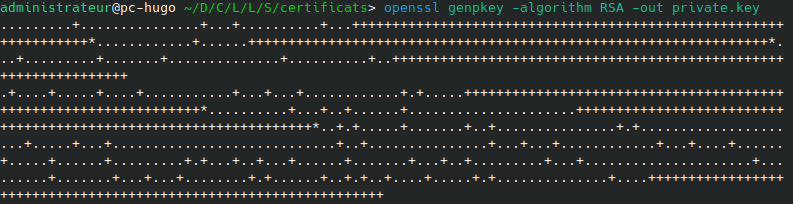
\includegraphics[scale=.85]{generation_key.png}
		\caption{Étapê 1 - Génération de la clé privée} 
	\end{center}
\end{figure}	

\begin{figure}[!h]
	\begin{center}
		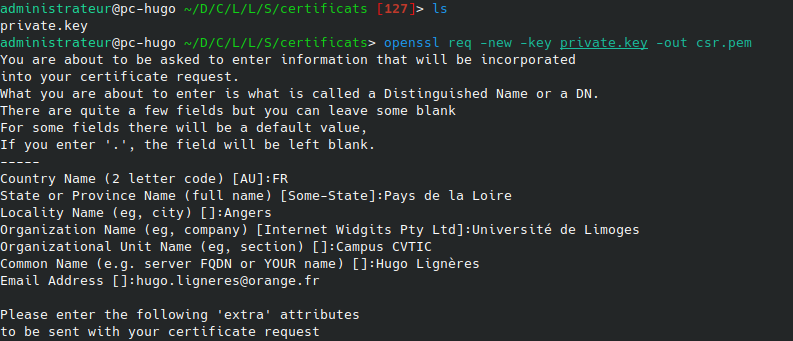
\includegraphics[scale=.85]{clee_privee.png}
		\caption{Étape 2 - Génération de demande de signature du certificat}
	\end{center}
\end{figure}	

\begin{figure}[!h]
	\begin{center}
		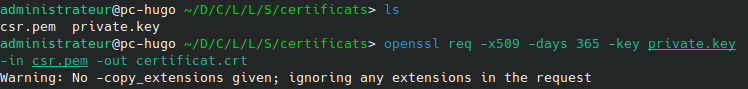
\includegraphics[scale=.85]{generation_certificat.png}
		\caption{Étape 3 - Génération d'un certificat auto-signé}
	\end{center}
\end{figure}	


	\subsection{Détails du certificat}

\begin{figure}[!h]
	\begin{center}
		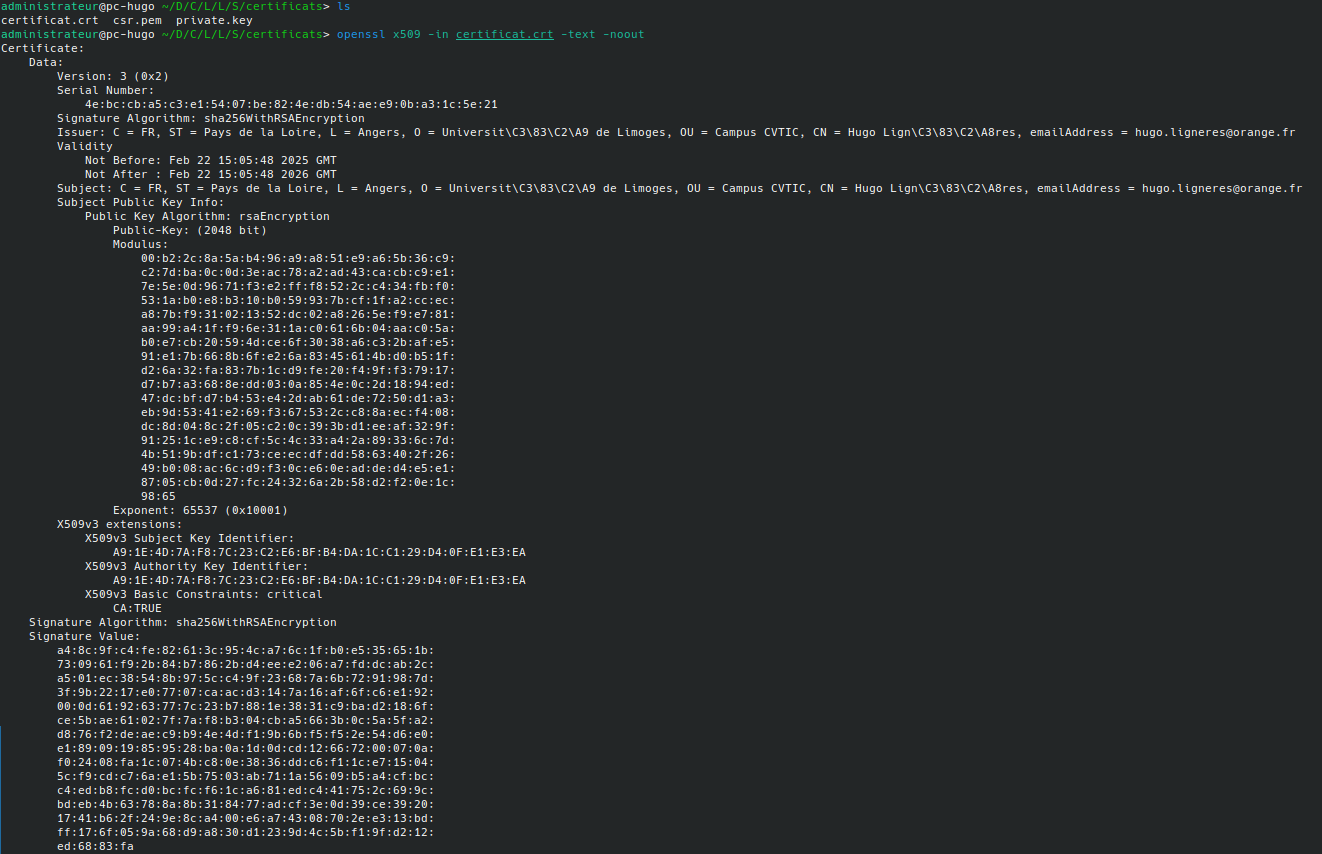
\includegraphics[scale=.5]{certificat_details.png}
		\caption{}
	\end{center}
\end{figure}	

Explication des détails du certificat : \\

\begin{itemize}
	\item \textbf{Version: 3 (0x2)} $\rightarrow$ 
	\item \textbf{Serial number} $\rightarrow$ numéro de série unique du certificat ;
	\item \textbf{Signature algorithm} $\rightarrow$ Algorithme de signature du certificat, qui est l'algorithme \texttt{SHA-256} avec RSA ;  
	\item \textbf{Issuer} $\rightarrow$ L'émetteur du certificat. Les détails affichés correspondent aux informations entrées pendant la génération de demande de signature du certificat ;
	\item \textbf{Validity} $\rightarrow$ Date jusqu'à laquelle le certificat sera valide et accepté par des applications utilisant SSL/TLS ;
	\item \textbf{Subject} $\rightarrow$ C'est l'identité du propriétaire du certificat. Comme il est auto-signé, le sujet est identique à l'émétteur ;
	\item \textbf{Public Key Algorithm: rsaEncryption} $\rightarrow$ L'algorithme utilisé pour chiffrer la clé publique ;
	\item \textbf{Public-Key: (2048 bit)} $\rightarrow$ La taille de l'algorithme ;
	\item \textbf{Modulus} $\rightarrow$ Partie publique de la clé RSA du certificat
	\item \textbf{Exponent} $\rightarrow$ Exposant utilisé dans le chiffrement RSA ;
	\item \textbf{X509v3 Subject Key Identifier} $\rightarrow$  Identifiant unique de la clé du sujet ;
	\item \textbf{X509v3 Authority Key Identifier} $\rightarrow$ Identifiant unique de la clé d'autorité. Identique à la clé du sujet car c'est une certificat auto-signé ;
	\item \textbf{CA:TRUE} $\rightarrow$ Indique que le certificat est un certificat d'autorité de certification :
	\item \textbf{Signature Algorithm: sha256WithRSAEncryption} $\rightarrow$ Indique que le certificat est chiffré et signé avec SHA-256 et RSA ;
	\item \textbf{Signature Value} $\rightarrow$	Signature permettant de vérifier l'authenticité du certificat.
	\end{itemize}

	\subsection{Comparaison entre deux certificats}

\begin{figure}[!h]
    \centering
    \begin{minipage}{0.3\textwidth}
        \centering
        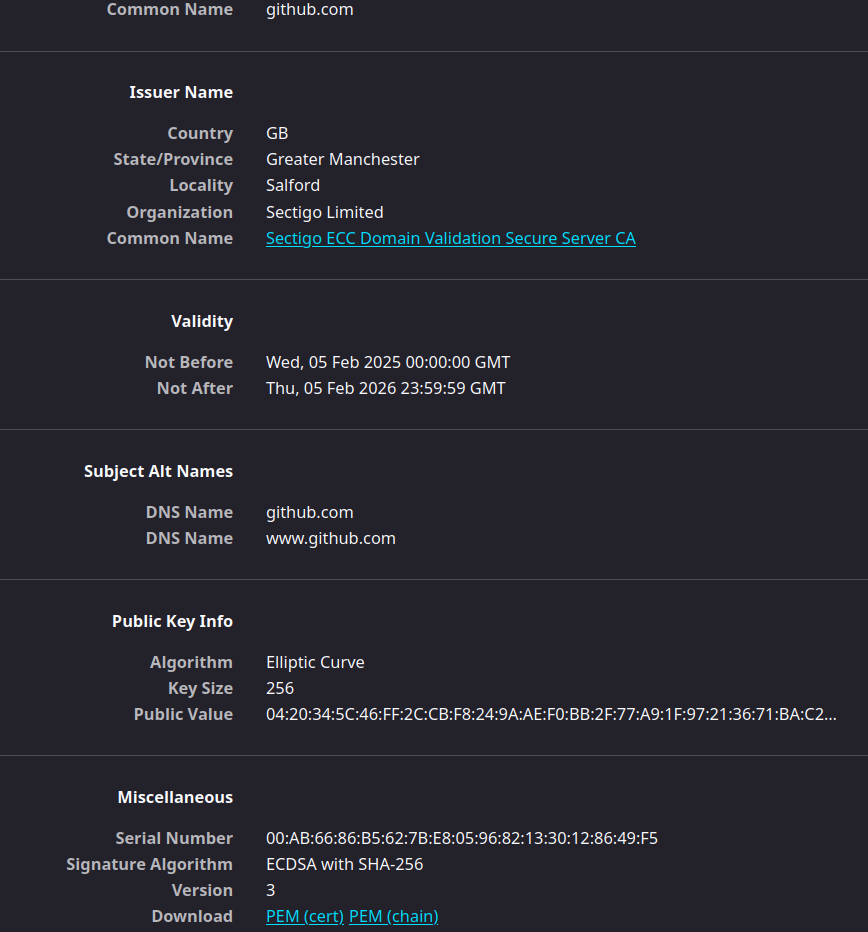
\includegraphics[scale=0.22]{github_1.png}
    \end{minipage}
    \begin{minipage}{0.3\textwidth}
        \centering
        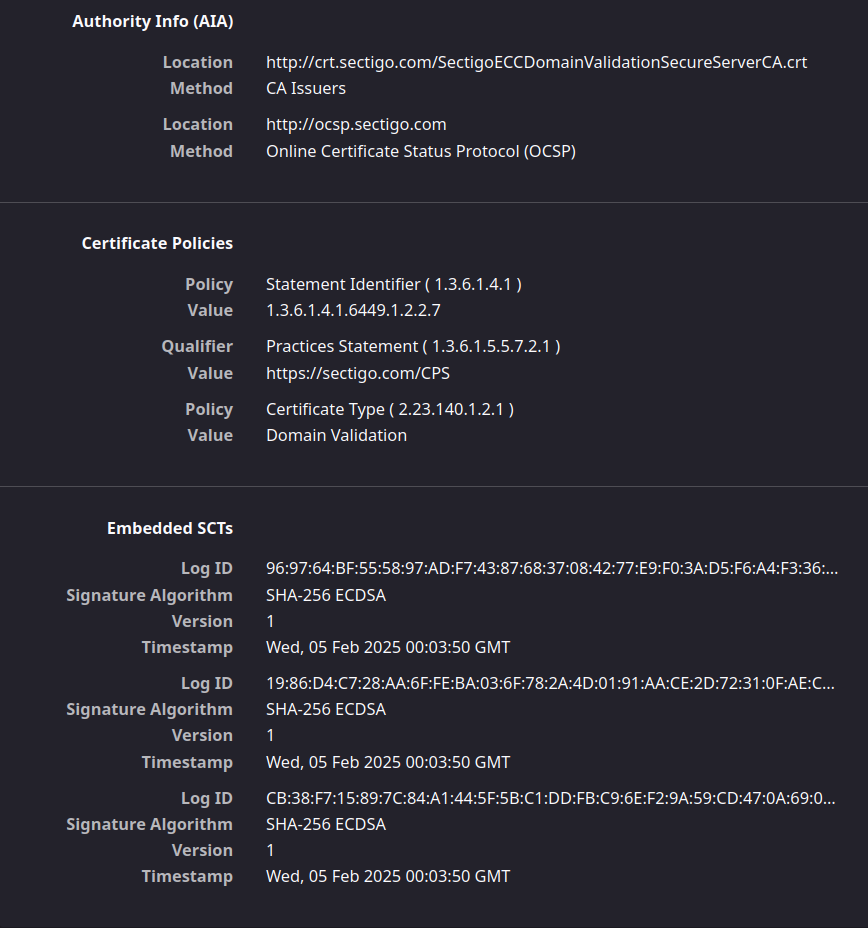
\includegraphics[scale=0.22]{github_3.png}
    \end{minipage}
    \begin{minipage}{0.3\textwidth}
        \centering
        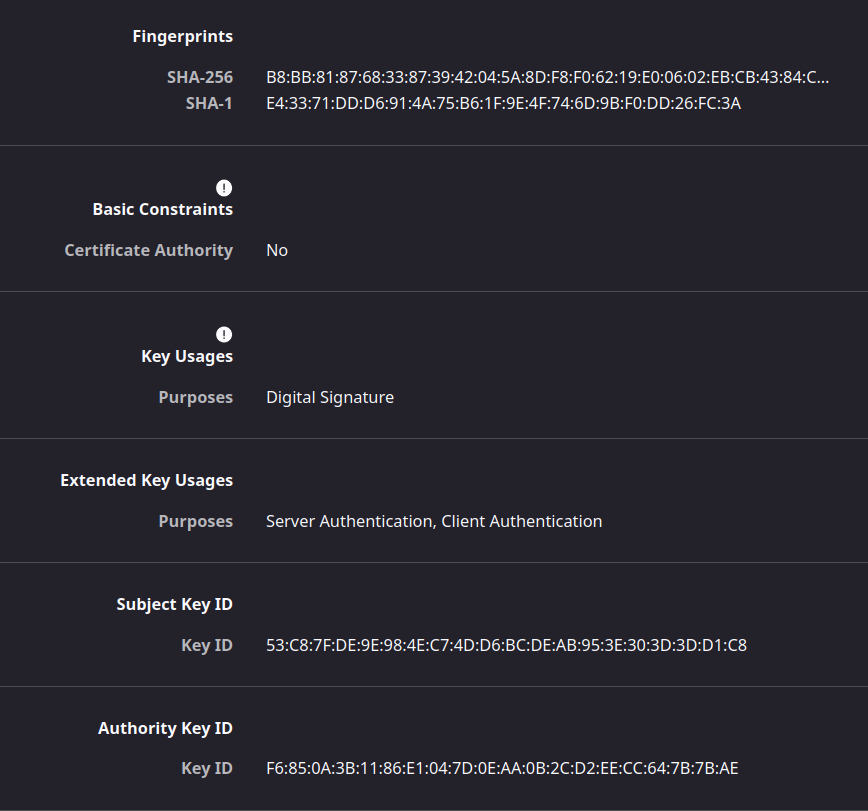
\includegraphics[scale=0.25]{github_2.png}
    \end{minipage}
    \caption{Certificat du site github.com}
\end{figure}

\begin{table}[!h]
	\centering
		\begin{tabular}{|c|c|c|}
			\hline
			& &\\
			\textbf{Élément} & \textbf{Certificat auto-signé} & \textbf{Certificat github.com} \\ 
			& &\\ \hline
			& & \\
			\textbf{Algorithme de signature} & SHA-256 avec RSA & SHA-256 avec ECDSA \\ 
			& &\\ \hline
			& &\\
			\textbf{Émetteur = Sujet ?} & Oui & Non \\ 
			& &\\ \hline
			& &\\
			\textbf{Algorithme clé publique} & rsaEncryption 2048 bit & Elliptic Curve - 256 bit\\ 
			& &\\ \hline
			& &\\
			\textbf{Algorithme de signature} & SHA-256 et RSA & SHA-256 ECDSA \\
			& &\\ \hline
			& &\\
			\textbf{Certificat d'autorité ?} & Oui & Non \\ 
			& &\\ \hline
			& &\\
			\textbf{Version} & 3 & 3 \\ 
			& &\\ \hline
		\end{tabular}
	\caption{Comparaison entre deux certificats}
\end{table}	


\newpage

\section{Recommandations ANSSI sur l'utilisation du protocole HTTPS}
 
	\begin{itemize}
		\item[1.] TLS : \begin{itemize}
			\item[-] Utiliser les versions 1.2 ou 1.3 ;
			\item[-] Éviter les connexions HTTP non-sécurisées en les redirigeant vers un HTTPS ;
			\item[-] Même si le site ne traite pas d'informations sensibles, toujours appliquer des recommandations de sécurité liées au TLS. \\
		\end{itemize}
		
		\item[2.] Mettre en œuvre le HTTP Strict Transport Security (HSTS) : \begin{itemize}
			\item[-] Activer l'HSTS pour forcer l'utilisation du HTTPS ;
			\item[-] Assurer que l'accès HTTPS est pérenne, car l'HSTS rend impossible l'accès en HTTP une fois activé ; \\
		\end{itemize}
		
		\item[3.] Surveiller les Certificate Transparency (CT) logs : \begin{itemize}
			\item[-] Mettre en place un processus de surveillance des CT logs pour détecter et révoquer les certificats illégitimes ;
			\item[-] Utiliser ces registres cryptographiquement sécurisés pour vérifier la légitimité des certificats émis par les autorités de certification.
		\end{itemize}
	\end{itemize}
	
	\subsection{Explication de certaines notions}
	
	\subsection{L'HTTP Strict Transport Security}
	
	L'HSTS est un mécanisme qui force l'utilisation du protocole HTTPS sur un site, en empêchant les navigateurs d'y accéder via un protocole HTTP non sécurisé. 
	
	Lorsqu'un navigateur accède à un site pour la première fois en HTTPS, le serveur envoi un en-tête HSTS dans sa réponse HTTP. Cet en-tête indique que toutes les connexions futures à ce site devront se faire en HTTPS, sinon le site ne sera pas accessible, ou le redirigera en HTTPS.
	
	\subsection{Certificate Transparency Logs}
	
	C'est un protocole dont le but est d'améliorer la sécurité et la transparence des certificats HTTPS, en mettant en place une journalisation qui produit des logs publiques des certificats SSl/LTS, délivrés par les autorités de certification.
	
	Lorsqu'une autorité de certification délivre un certificat, elle ajoute ce dernier dans un CT log. Chaque certificat ajouté aux logs est enregistré de manière sécurisée. Pourquoi c'est utile? Parce que les navigateurs exigent que les sites en HTTPS utilisent des certificats enregistrés dans les logs. Également, un site peut surveiller ces logs pour s'assurer qu'il n'y a pas de faux certificats.

\newpage
	
	
\section{Ressources utilisées}

	\subsection*{Sources}

	\begin{itemize}
		\item \url{https://www.technologygee.com/what-is-the-domain-name-system-dns-protocol/}
		\item \url{https://next.ink/28083/82009-le-new-york-times-et-twitter-victimes-hier-soir-dun-detournement-dns/}
		\item \url{https://www.frameip.com/dns/#61-8211-fragilite}
		\item \url{https://www.ibm.com/fr-fr/topics/dns-protocol}
		\item \url{https://fr.wikipedia.org/wiki/Domain_Name_System}
		\item \url{https://www.nameshield.com/ressources/lexique/dns-domain-name-system/}
		\item \url{https://www.paloaltonetworks.com/cyberpedia/what-is-a-dns-attack}
	\end{itemize}


\end{document}
